% !TeX root = ../main.tex

\chapter{Device fabrication of silicon nitride ring resonators}

Different from fabrication of silicon-on-insulator, which is CMOS-compatible and fully understood both in the laboratory and semiconductor industry, fabricating integrated silicon nitride device, in particular high Q-factor ring resonators, is only realized in several group all around the word. 

Collaborating with Yokoyama Lab in Kyushu University, we perform the subtractive fabrication of silicon nitride ring resonators, along with other optical devices. To discover the diversity of fabrication recipes and compare the material properties, we also design the device layout and order the devices using ligentec process and NTT-AT process.

\section{Subtractive fabrication process}

The subtractive fabrication of waveguide is widely perform in a variety of material platforms, including silicon nitride. The previous work concerning our fabrication processes reported ring resonators with high \textit{Q}-factor up to \num{5.2d4} and waveguides with measured loss of 2.9 dB/cm \cite{Cheng2017b}. 

\begin{figure}
	\centering
	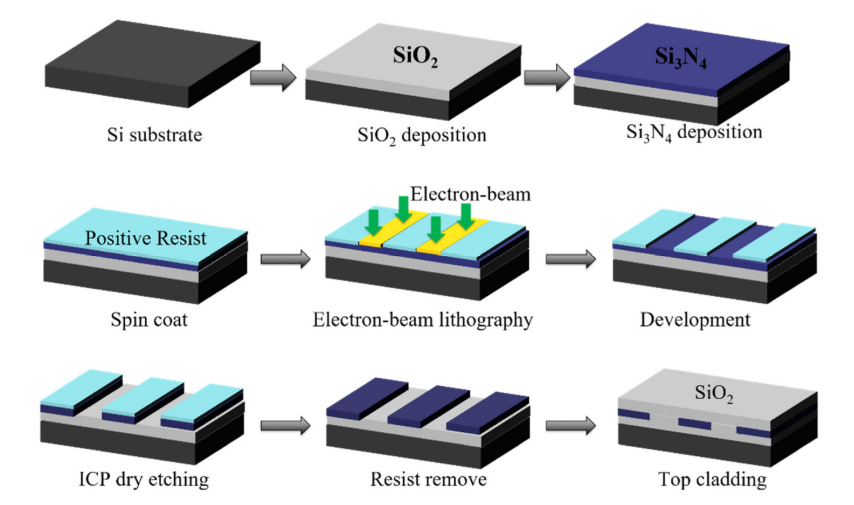
\includegraphics[width=1.0\linewidth]{imgs/png/fab-flow}
	\mycaption{Schematic process flow of the subtractive process}{}
	\label{fig:fab-flow}
\end{figure}

The schematic process flow of the subtractive process is shown in \autoref{fig:fab-flow}. 

To begin this process, we deposit the silicon dioxide over a 4 inch silicon wafer using the TEOS source or begin with a thermal oxidized wafer. The film

Recently, Si3N4 has been widely utilized in integrated optic devices because of its conspicuous flexibility in the refractive index around 2.0. In our fabrication (Fig. 1), the Si3N4 films with controlled thickness and refractive index were deposited onto the SiO2/Si substrate through LSCVD using the liquid SiN-X source (SAMCO Inc.) with N2 or N2O. The measured refractive index of the deposited Si3N4 film was 1.99, which can be turned to between 1.66 and 1.78 as silicon oxynitride (SiOxNy) by mixing N2O gas. The propagation loss of the films also demonstrated a temperature dependence of the deposition. If the temperature is set too low, the chemical reaction may be uncompleted to form Si3N4. We found that the optimal deposition temperature was 150C to obtain the required low loss properties. The photonic patterns of waveguides, ring resonators, and grating couplers were transferred onto the resist
layer on Si3N4 by using the electron beam lithography (EBL) technique. The direct write capability of EBL guarantees the small feature size and high accuracy of the device. After development, the patterned resist was hard-baked at 150C for 5 minutes. This process is effective to improve the dry etching selectivity of the resist and Si3N4, and to help to achieve rectangle waveguide cross-sections. We used a mixed gas of CHF3/O2 for the inductively coupled plasma reactive ion etching (ICP-RIE). After etching to reach the desired depths, we striped the leftover resist using the RIE in which the O2 plasma removes only the resist, but leaves the exposed Si3N4 waveguide untouched. By utilizing CVD, we deposited a top cladding of SiO2 onto the Si3N4 core to form a buried ridge waveguide resonator

\subsection{Film deposition}
\subsection{Material properties}
\subsection{Patterning and etching}
\subsection{Top-cladding and annealing}
\subsection{Optical I/O and packaging}

\section{Fabless samples via foundries}

\subsection{Ligentec}

\subsection{NTT-AT}

